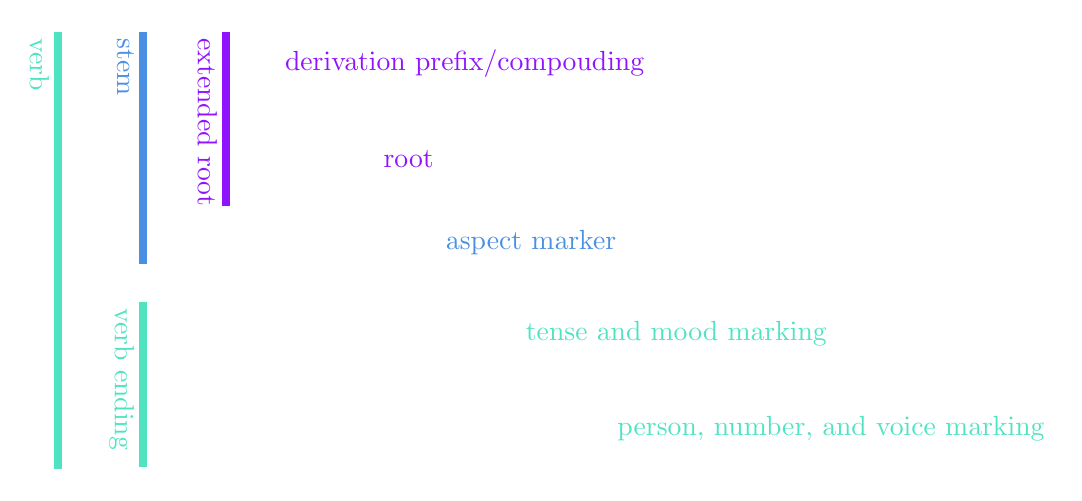
\begin{tikzpicture}[x=0.75pt,y=0.75pt,yscale=-1,xscale=1]
    %uncomment if require: \path (0,340); %set diagram left start at 0, and has height of 340
    
    %Straight Lines [id:da11881532570567654] 
    \draw [color={rgb, 255:red, 144; green, 19; blue, 254 }  ,draw opacity=1 ][fill={rgb, 255:red, 144; green, 19; blue, 254 }  ,fill opacity=1 ][line width=3]    (160,37.93) -- (160,121.93) ;
    %Straight Lines [id:da5525279444002422] 
    \draw [color={rgb, 255:red, 74; green, 144; blue, 226 }  ,draw opacity=1 ][fill={rgb, 255:red, 144; green, 19; blue, 254 }  ,fill opacity=1 ][line width=3]    (120,37.93) -- (120,149.93) ;
    %Straight Lines [id:da5129611438909998] 
    \draw [color={rgb, 255:red, 80; green, 227; blue, 194 }  ,draw opacity=1 ][fill={rgb, 255:red, 144; green, 19; blue, 254 }  ,fill opacity=1 ][line width=3]    (120,167.93) -- (120,247.59) ;
    %Straight Lines [id:da013912639121147041] 
    \draw [color={rgb, 255:red, 80; green, 227; blue, 194 }  ,draw opacity=1 ][fill={rgb, 255:red, 144; green, 19; blue, 254 }  ,fill opacity=1 ][line width=3]    (79,37.93) -- (79,248.59) ;
    
    % Text Node
    \draw (157,39.93) node [anchor=north west][inner sep=0.75pt]  [color={rgb, 255:red, 144; green, 19; blue, 254 }  ,opacity=1 ,rotate=-90] [align=left] {extended root};
    % Text Node
    \draw (117,169.93) node [anchor=north west][inner sep=0.75pt]  [color={rgb, 255:red, 80; green, 227; blue, 194 }  ,opacity=1 ,rotate=-90] [align=left] {verb ending};
    % Text Node
    \draw (275,53.24) node  [color={rgb, 255:red, 144; green, 19; blue, 254 }  ,opacity=1 ] [align=left] {derivation prefix/compouding};
    % Text Node
    \draw (248.01,99.24) node  [color={rgb, 255:red, 144; green, 19; blue, 254 }  ,opacity=1 ] [align=left] {root};
    % Text Node
    \draw (307.01,139.24) node  [color={rgb, 255:red, 74; green, 144; blue, 226 }  ,opacity=1 ] [align=left] {aspect marker};
    % Text Node
    \draw (377.01,183.24) node  [color={rgb, 255:red, 80; green, 227; blue, 194 }  ,opacity=1 ] [align=left] {tense and mood marking};
    % Text Node
    \draw (451.51,229.24) node  [color={rgb, 255:red, 80; green, 227; blue, 194 }  ,opacity=1 ] [align=left] {person, number, and voice marking};
    % Text Node
    \draw (117,39.93) node [anchor=north west][inner sep=0.75pt]  [color={rgb, 255:red, 74; green, 144; blue, 226 }  ,opacity=1 ,rotate=-90] [align=left] {stem};
    % Text Node
    \draw (76,39.93) node [anchor=north west][inner sep=0.75pt]  [color={rgb, 255:red, 80; green, 227; blue, 194 }  ,opacity=1 ,rotate=-90] [align=left] {verb};
    
    
    \end{tikzpicture}
    